\subsection{Kühlung}\label{sec: Kühlung}
In der Testkammer kann es sehr warm werden, weshalb eine Regelung der Temperatur wichtig ist. Diese erfolgt durch den Einsatz eines Kühlgeräts. Die Suche nach einem passenden Kühlgerät gestaltete sich jedoch schwierig, da es spezifische Anforderungen erfüllen musste: Es war notwendig, dass das Gerät über analoge Knöpfe verfügt. Der Grund dafür liegt in der Notwendigkeit, dass wir es zunächst über einen Arduino und später über einen Raspberry Pi steuern können.\\
\subsubsection{Verkabelung des Kühlgerät}
\begin{figwindow}[0,r,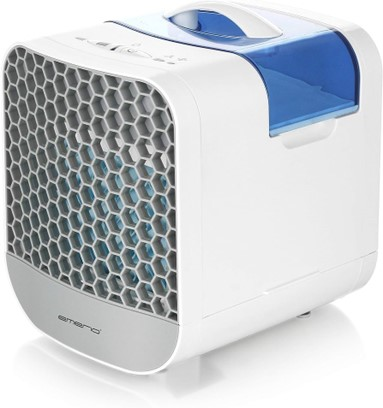
\includegraphics[scale=0.6]{image/kühlgerät.jpg},{Kühlgerät mit analogen Knöpfen\autocite{Kuehlung}}]
Abbildung zeigt das Kühlgerät mit den analog zu bedienenden Knöpfe.\\

Das Gerät ist auch ohne die Zugabe von Wasser als Ventilator nutzbar.\\

Es gibt zwei verschiedene Geschwindigkeitsstufen.\\

Das in Abbildung 63 gezeigte Kühlgerät konnte durch einige Modifikationen von einem Raspberry Pi bzw. einem Arduino angesteuert werden.
\end{figwindow}
\vspace{3mm}
Der Luftkühler:
\begin{itemize}
    \item Der Luftkühler verfügt über einen Ventilator, der warme Luft ansaugt und sie im Inneren des Gerätes durch einen mit Wasser befeuchteten Filter befördert. Dadurch wird die warme Luft effizient abgekühlt und tritt wieder aus dem Gerät aus. Eine angenehm kühle Brise entsteht.
\end{itemize}
\pagebreak
Wassertank:
\begin{itemize}
    \item Der blaue Wassertank ist entnehmbar. Man kann den Wassertank am Griff aus dem Gerät entnehmen und somit sehr einfach mit frischem Wasser nachfüllen. Der Wassertank hat ein Volumen von 0,75 Litern.
\end{itemize}
\vspace{3mm}
\begin{figure}[H]
    \centering
    \includegraphics[scale=0.8]{image/auseinanderkühlung.jpg}
    \caption{Auseinandergebautes Kühlgerät}
    \label{fig:enter-label}
\end{figure}
\vspace{3mm}
Abbildung zeigt die zwei Taster für die Steuerung des Kühlgerätes. Der linke Taster steuert die 2 Stufen des Kühlgerätes und der rechte Taster dient zur Befeuchtung des Filters.\\

\newpage
\subsubsection{Verdrahtung der Taster}
\begin{figwindow}[0,l,\includegraphics[scale=0.8]{image/verkabelnkühlung.jpg},{Verkabeltes Kühlgerät für Lüftungsstufen}]
Der Taster wird nun verdrahtet. Jeweils eine Verbindung besteht vom Anschluss 1 zum Anschluss 2 und von Anschluss 3 zum Anschluss 4. Vom Anschluss 2 führt eine Verbindung über den Widerstand zum Mikrocontroller.\\

Der gleiche Vorgang muss auch für den 2. Schalter durchgeführt werden.

\end{figwindow}
\vspace{40mm}
Die rote Leitung ist Vin, diese Leitung ist allerdings nur kurz zu Testzwecken verwendet worden. Da der Arduino per USB mit Strom versorgt wird, ist die Vin Leitung nicht notwendig.

\subsubsection{Aufbau mittels Streifenrasterplatine}
\begin{figure}[H]
    \centering
    \includegraphics[scale=0.9]{image/streifenrasterkühl.png}
    \caption{Aufbau Streifenrasterplatine (Kühlgerät)}
    \label{fig:enter-label}
\end{figure}
\vspace{3mm}
\begin{figure}[H]
	\centering
	\includegraphics[scale=0.8]{image/gehäusestreifen.png}
	\caption{Halterung der Streifenrasterplatine}
	\label{fig:enter-label}
\end{figure}
Die Grundfläche der Halterung besteht aus einem 3,2 cm x 3,2 cm großem Quadrat, wie die Abbildung 22 zeigt. Damit die Halterung am Kühlgerät abgeschraubt werden kann, falls dies notwendig ist, habe ich die vier Löcher seitlich an der Halterung gemacht.\\
\vspace{3mm}
\begin{figure}[H]
    \centering
    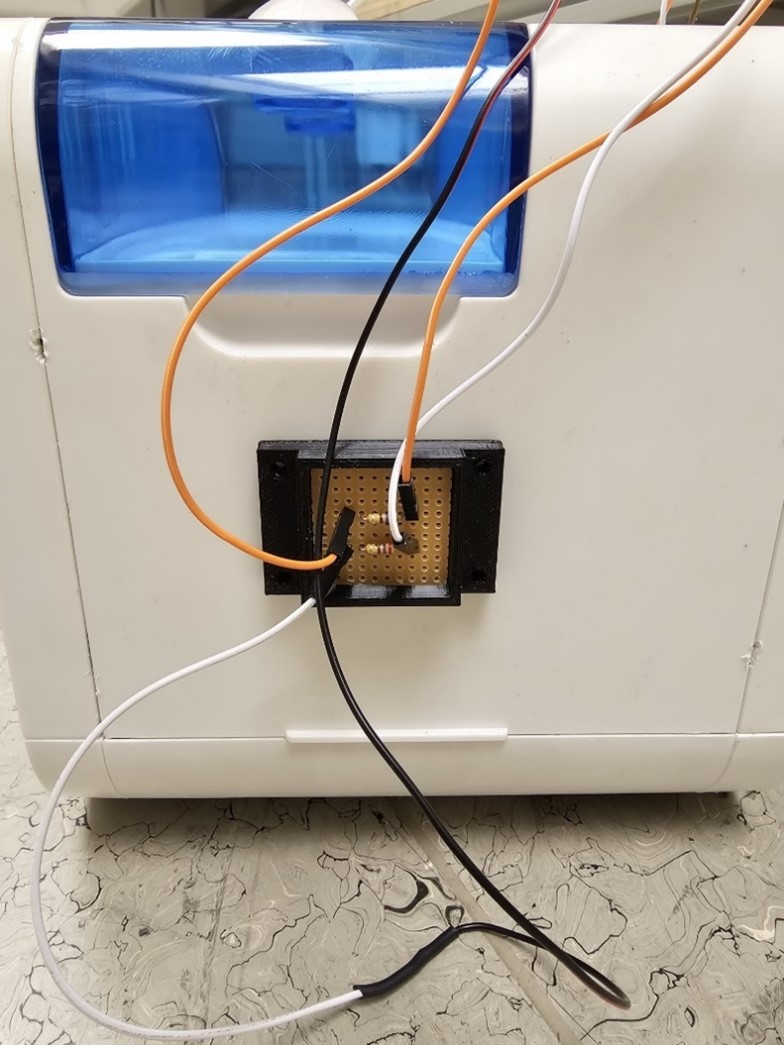
\includegraphics[scale=0.7]{image/streifenanbringen.jpg}
    \caption{Anbringen der Streifenrasterplatine am Kühlgerät}
    \label{fig:enter-label}
\end{figure}
Für die Streifenrasterplatine wurde eine Halterung mit dem 3D-Drucker gefertigt. Diese wurde mittels doppelseitigem Klebeband. Am Kühlgerät angebracht. Die Halterung wurde nicht wie ursprünglich geplant angeschraubt, da das Gehäuse des Kühlgeräts nicht beschädigt werden soll.
\newpage
\subsubsection{Befestigung des Kühlgeräts an der Teststation}

Damit das Kühlgerät die Testkammer kühlen kann, muss an der Rückseite der Testkammer ein Loch eingesägt werden. Die Maße des Loches in der PVC-Platte müssen genau mit denen vom Kühlgerät übereinstimmen, damit das Kühlgerät fest darin verankert wird.\\
\vspace{3mm}
%width=\textwidth

\vspace{3mm}


\begin{figure}[H]
	\centering
	\begin{subfigure}[b]{0.5\textwidth}
		\centering
		\includegraphics[scale=0.8]{image/kühlung1.png}
		\caption{Loch in der PVC-Platte}
		\label{fig:bild1}
	\end{subfigure}
	\hfill
	\begin{subfigure}[b]{0.5\textwidth}
		\centering
		\includegraphics[scale=1.1]{image/kühlung2.png}
		\caption{Befestigung des Kühlgeräts auf der Rückseite}
		\label{fig:bild2}
	\end{subfigure}
	\caption{Kühlung in der Teststation}
	\label{fig:zwei_bilder}
\end{figure}